\documentclass{article}
\usepackage{graphicx}
\usepackage[utf8]{inputenc}
\usepackage{fullpage}
\usepackage{listings}
\usepackage{xcolor}
\usepackage{url}
\usepackage[linesnumbered,ruled,vlined]{algorithm2e}
\usepackage{enumitem}
\usepackage{mathtools}
\usepackage{amssymb}
\usepackage{amsthm}
\renewcommand*{\proofname}{Prova}


\DeclarePairedDelimiter\ceil{\lceil}{\rceil}


\parindent0in
\pagestyle{plain}
\thispagestyle{plain}
\setlength{\parskip}{1em}

\newcommand{\assignment}{Homework 1}
\newcommand{\duedate}{July 21, 2019}

% \renewcommand\thesubsection{\arabic{subsection}}

\title{Homework 1}
\date{20/07/2019}

\begin{document}

Fundação Getulio Vargas\hfill\\
Estruturas de Dados e Algoritmos\hfill\textbf{\assignment}\\
Prof.\ Jorge Poco\hfill\textbf{Due}: \duedate\\
Aluno: Davi Sales Barreira
\smallskip\hrule\bigskip

{\let\newpage\relax\maketitle}
\maketitle


\section{Induction [3pts]}
Answers should be written in this document. 

\begin{enumerate}
  \item Prove by Induction that:
  \( \sum_{i=1}^{n}i^2=\frac{n(n+1)(2n+1)}{6} \qquad\forall n \geq 0\)

  \item Prove by Induction that:
  $\forall n \geq 7$ it is true $3^n<n!$
  
  \item Prove by Induction that $\forall n \geq 0$
  \[
    \left \lceil\frac{n}{2} \right \rceil=
    \left\{
    \begin{array}{ll}
    \frac{n}{2}& \textrm{si $n$ es par}\\
    \frac{n+1}{2}& \textrm{si $n$ es impar}
    \end{array}
    \right.
  \]
  
    \item Prove by induction that a number is divisible by 3 if and only if the sum of its digits is divisible by 3.
    
    \item Prove that any integer greater than 59 can be formed using only 7 and 11 cent coins.
  
  \item Prove by induction that $F_{n+k}=F_{k}F_{n+1}+F_{k-1}F_{n}$
  
  \item Prove by induction in $n$ that \(\sum_{m=0}^{n}{n \choose m}=2^n\)
  
  \item Prove by induction that a graph with $n$ vertices can have at most  $\frac{n(n-1)}{2}$ edges.
  
  \item Prove by induction that a complete binary tree\footnote{http://web.cecs.pdx.edu/~sheard/course/Cs163/Doc/FullvsComplete.html} with $n$ levels has $2^n-1$ vertices.
  
  \item A polygon is convex if each pair of points in the polygon can be joined by a straight line that does not leave the polygon. Prove by induction in $n>3$ that the sum of the angles of a polygon of $n$ vertices is $180(n-2)$.
  
\end{enumerate}

\section{Correctness of bubblesort [2pts]}
Bubblesort is a popular, but inefficient, sorting algorithm. It works by repeatedly swapping adjacent elements that are out of order.

\begin{algorithm}[H]
\SetAlgoLined
  \For{$i = 1$ \textbf{to} $A.length -1$} {
    \For{$j = A.length$ \textbf{downto} $i + 1$} {
      \If{$A[j] < A[j-1]$} {
        exchange $A[j]$ with $A[j-1]$
      }
    }
  }
\caption{BUBBLESORT(A)}
\end{algorithm}

\begin{enumerate}[label=\Alph*]
  \item Let $A'$ denote the output of BUBBLESORT(A). To prove that BUBBLESORT is correct, we need to prove that it terminates and that
  
  \begin{equation} \label{eq:1}
    A'[1] \leq A'[2] \leq ... \leq A'[n]
  \end{equation}
  
  where $n = A.length$. In order to show that BUBBLESORT actually sorts, what else do we need to prove?
  
  The next two parts will prove inequality~(\ref{eq:1}).
  
  \item State precisely a loop invariant for the \textbf{for} loop in lines 2–6, and prove that this loop invariant holds. Your proof should use the structure of the loop invariant proof presented in this chapter.
  
  \item Using the termination condition of the loop invariant proved in part (B), state a loop invariant for the for loop in lines 1–7 that will allow you to prove inequality~(\ref{eq:1}). Your proof should use the structure of the loop invariant proof presented in this chapter.
  
  \item What is the worst-case running time of BUBBLESORT? How does it compare to the running time of insertion sort?
\end{enumerate}


\section{Growth of Functions [2pts]}

\begin{enumerate}[label=\Alph*]
  \item For each of the following pairs of functions, either $f(n)$ is in $O(g(n))$, $f(n)$ is in $\Omega(g(n))$, or $f(n) = \Theta(g(n))$. Determine which relationship is correct and briefly explain why.
    \begin{itemize}
      \item $f(n) = \log n^2$; $g(n) = \log n + 5$
      \item $f(n) = \log^2 n$; $g(n) = \log n$
      \item $f(n) = n\log n + n$; $g(n) = \log n$
      \item $f(n) = 2^n$; $g(n) = 10n^2$
    \end{itemize}
  
  \item Prove that $n^3 -3n^2 -n+1 = \Theta(n^3)$.
  \item Prove that $n^2 = O(2^n)$.
  
\end{enumerate}


\section{Insertion Sort - Mergesort - Quicksort [3pts]}
Implement the insertion sort, merge sort and quicksort using the template \texttt{test.py} (use Python 3.X). Create a \texttt{test.cpp} file and write the equivalent code from \texttt{test.py} in C++, ie., the functions: main, \texttt{insertion\_sort}, \texttt{merge\_sort}, \texttt{quicksort} and \texttt{is\_sorted}. For the random number generations you can use the \texttt{rand} function from \texttt{cstdlib}\footnote{\url{http://www.cplusplus.com/reference/cstdlib/rand/}}. Your code should print the tuple (number of objects, time insertion\_sort, time merge\_sort, time quicksort)

You must submit both \texttt{test.py} and \texttt{test.cpp}. Graphs and descriptions must be included in this document. 

\subsection{Random Order}
\begin{enumerate}
  \item Create 10 sets of numbers in random order. The sets must have \{10k, 20k, 30k, ..., 100k\} numbers.
  
  \item Sort these numbers using the 3 algorithms and calculate the time each algorithm takes for each set of numbers.
  
  \item Generate a plot (using excel or another tool) showing a \emph{linechart}, where the $x$-axis is the ``number of elements", and the $y$-axis is the time that the algorithms took in C++ and Python. This plot must have 6 lines of different colors with a legend.
  
  \item Write a small paragraph (3 to 4 lines) describing the results.

\end{enumerate}

\subsection{Ascending Order}
Do the same experiment when the numbers are ordered in ascending order.

\subsection{Descending Order}
Do the same experiment when the numbers are ordered in descending order.

\pagebreak
\part*{Respostas}

\section*{Questão 1}
\subsection*{1.1}
\begin{proof}
$ $\newline
Caso Base: $n = 1$, temos $\sum^{n}_{i=1}{i^2}= \frac{1\cdot2\cdot3}{6}=1 \therefore$ Satisfeito para $n = 1$.

Hipótese indutiva: Supondo que $\sum^{n}_{i=1}{i^2} =\frac{n(n+1)(2n+1)}{6}$, para $n = k$.

Passo de indução: Seja $n = k + 1$
$$\sum^{k+1}_{i=1}{i^2} = (k+1)^2 + \frac{k(k+1)(2k+1)}{6} =
\frac{(k+1)(6(k+1) + k(2k + 1))}{6} = \frac{(k+1)(k+2)(2k +3)}{6} 
$$
$$
\sum^{k+1}_{i=1}{i^2} = \frac{(k+1)(k+1+1))(2(k+1)+1)}{6}
$$
\end{proof}

\subsection*{1.2}
\begin{proof}
$ $\newline
Caso Base: $n = 7$, temos $n! = 7! = 5040$ e $3^7 = 2187 \therefore$ Satisfeito para $n = 7$.

Hipótese indutiva: Supondo que para $n=k, 3^k < k!$

Passo de indução: Seja $n = k + 1$, $3^k < k!$
, note que como $k>3$, temos que $k+1>3$

$\therefore 3^{k+1}=3^k\cdot3 < k!\cdot(k+1)=(k+1)!$

\end{proof}

\subsection*{1.3}
\begin{proof}
$ $\newline
  \[Prop:
    \left \lceil\frac{n}{2} \right \rceil=
    \left\{
    \begin{array}{ll}
    \frac{n}{2}& \textrm{se $n$ é par}\\
    \frac{n+1}{2}& \textrm{se $n$ é impar}
    \end{array}
    \right.
  \]
\end{proof}

\begin{proof}
$ $\newline
Caso Base: 

$n=0,\lceil\frac{0}{2}\rceil=0=\frac{n}{2}\therefore$ satisfeito para $n=0$

$n=1,\lceil\frac{1}{2}\rceil=1=\frac{1+1}{2}\therefore$ satisfeito para $n=1$

Hipótese indutiva: Supondo que para $n=k$ vale a proposição.

Passo de indução: Se $k$ for par, então $\lceil\frac{k}{2} \rceil = \frac{k}{2}$, assim
$k+1$ é ímpar, logo
$$
\ceil*{\frac{n+1}{2}} = \ceil*{\frac{k}{2}} + \ceil*{\frac{1}{2}} =\frac{k}{2}+1 = \frac{(k+1)+1}{2}
$$
Se k for ímpar, $\ceil*{\frac{k}{2}} = \frac{k+1}{2}$, assim $k+1$ é par, logo
$$\ceil*{\frac{k+1}{2}}=\frac{k+1}{2}$$
\end{proof}


\subsection*{1.4}
\begin{proof}
Vamos provar que o resto da divisão de um número por 3 é igual ao resto da divisão da soma
dos seus dígitos, ou seja, em $P_n$ temos que $\overline{a_1a_2...a_n} \mod 3 = \sum_{i=1}^n{a_i} \mod 3$

Caso Base: Para $P_1$ temos os número com 1 dígito, portanto a condição é satisfeita trivialmente já
a soma dos dígitos é igual ao próprio número.

Hipótese indutiva: Supondo que $P_n$ é válida.

Passo de indução: Analisando $P_{n+1}$, temos então A = $\overline{a_1...a_na_{n+1}} = \overline{a_1...a_n}+10*a_{n+1}$:
$$A \mod 3 = \overline{a_1...a_{n+1}} \mod 3$$
$$A \mod 3 = \overline{a_0...a_n} + 10a_{n+1} \mod 3$$
$$A \mod 3 = \overline{a_0...a_n} + a_{n+1} +9a_{n+1} \mod 3$$
Como $9a_{n+1} \mod 3 = 0$, então, utilizando a propriedade $P_n$, temos que:
$$A \mod 3 = \overline{a_0...a_n} + a_{n+1} \mod 3 = a_0 + ... + a_n + a_{n+1} \mod 3$$
\end{proof}


\subsection*{1.5}
\begin{proof}
$ $\newline
Caso Base: $n = 60 = 7\cdot7 + 11\cdot1 \therefore$ Satisfeito. 

Hipótese indutiva: Supondo que para $n=k = a\cdot7 + b\dot11$, onde $a,b \in \mathbb{N}\cup\{0\}$

Passo de indução: Para $n = k+1$, temos que $k+1 =a\cdot7 + b\dot11 + 1$.

Utilizaremos o fato de que $2\cdot11-3\cdot7 = 1$ e $8\cdot7 - 5\cdot11 = 1$.

\begin{itemize}

\item Se $a >= 3 \therefore k + 1 =a\cdot7+b\cdot11+2\cdot11-3\cdot7 = (a-3)\cdot7 + (b+2)\cdot11$. Portanto,
a proposição vale quando $a >=3 $.

\item Se $a<3$, ou seja $a \in \{0,1,2\}$. Além disso, como $n > 59$ e $a\cdot7 + b\cdot11 > 59 \implies b > 4$, já que $a$ é no máximo 2.
Logo, podemos fazer:
$$k+1 =a\cdot7+b\cdot11+8\cdot11-3\cdot7 = (a+8)\cdot7 + (b-5)\cdot11 $$

\end{itemize}
\end{proof}

\subsection*{1.6}
\begin{proof}
$ $\newline
$F = Fibonacci \therefore F_3 = F_2 + F_1$, além disso, $F_1,F_2 = 1$

Caso Base:
\begin{itemize}
\item Para $n=1$, $F_{1+k}=F_k\cdot F_2+F_1\cdot F_{k-1}=F_k\cdot1+1\cdot F_{k-1} = F_{k+1} \therefore$ Satisfeito.

\item Para $n=2$, $F_{2+k}=F_k\cdot F_3+F_2\cdot F_{k-1}=F_k\cdot2+1\cdot F_{k-1} = F_k + F_k + F_{k-1} = F_k + F_{k+1} =F_{k+2} \therefore$ Satisfeito.
\end{itemize}

Hipótese indutiva: Supondo que $F_{n+k} = F_k \cdot F_{n+1} + F_{k-1} \cdot F_n$ e que $F_{n+k-1} = F_k \cdot F_{n} + F_{k-1} \cdot F_{n-1}$

Passo de indução: Sabemos que na sequência de Fibonacci $F{n+1+k} = F_{n+k} + F_{n-1+k}$, portanto,
$$F_{n+1+k} = F_k \cdot F_{n+1} + F_{k-1} \cdot F_n + F_k \cdot F_{n} + F_{k-1} \cdot F_{n-1}$$
$$F_{n+1+k} = F_k(F_{n+1}+F_{n})+F_{k-1}(F_n + F_{n-1}) = F_k\cdot F_{n+2}+F_{k-1}\cdot F_{n+1}$$

\end{proof}

\subsection*{1.7}
\begin{proof}
$ $\newline
Caso Base: $n = 1,\sum^1_{m=0}{n\choose m}={1\choose 0}+{0\choose 0}=2^1 \therefore$ Satisfeito.

Hipótese indutiva: Supondo que para $n=\sum^1_{m=0}{k\choose m}=2^k$

Passo de indução: Seja $n = k + 1$, utilizaremos a seguinte identidade ${k+1\choose m} = {k\choose m}+{k \choose m-1}$.
$$2\cdot \sum^k_{m=0}{k\choose m} = \bigg[\underbrace{{k\choose 0}}_{k+1\choose0}  + \underbrace{{k\choose 0}+{k\choose 1}}_{k+1\choose 1}
+{k\choose 1}+{k \choose 2}+...+
\underbrace{{k\choose k-1}+{k\choose k}}_{k+1\choose k}+\underbrace{{k\choose k}}_{k+1\choose k+1}\bigg]$$
$$2\cdot 2^k = \bigg[{k+1\choose0}+{k+1\choose1}+...+{k+1\choose k+1}\bigg] = \sum^{k+1}_{m=0}{k+1\choose m}$$

\end{proof}


\section*{Questão 2}
\section*{Questão 3}
\section*{Questão 4}

Os gráficos abaixo comparam os resultados obtidos para os diferentes algoritmos de sorting
implementados tanto em C++ como em Python, sendo os gráficos da direita em escala logaritmica para o eixo y.
Como esperado, o código de C++ performa melhor
que em Python, com a diferença maior sendo no algoritmo de {\it insert sort}.

Além disso, observamos que o {\it quicksort} apresentou o melhor
desempenho considerando tanto o vetor com valores aleatórios como o com
valores descendentes.
No vetor já ordenado ({\it ascending}), o tempo dos três algoritmos é muito baixo, como
era de se esperar, porém, nesse caso o {\it insert sort} foi quem apresentou o melhor
resultado.


  \begin{figure}[!h]
  \centering
  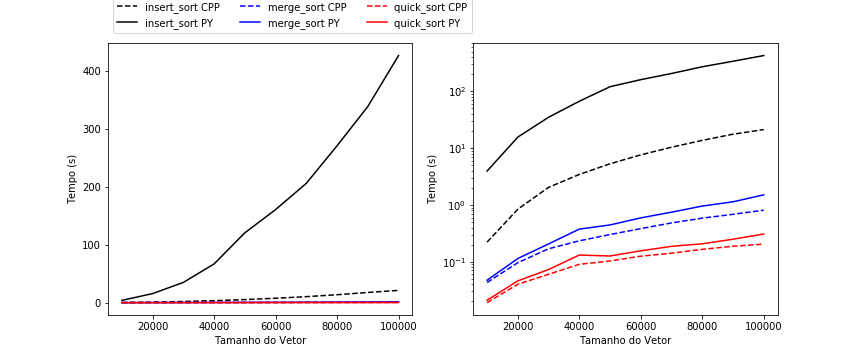
\includegraphics[width=0.8\linewidth,height=5cm]{SortTime_Random.png}
    \caption{Comparação de performance dos algoritmos de {\it sorting} para vetores aleatórios}
    \vspace{0.5cm}
  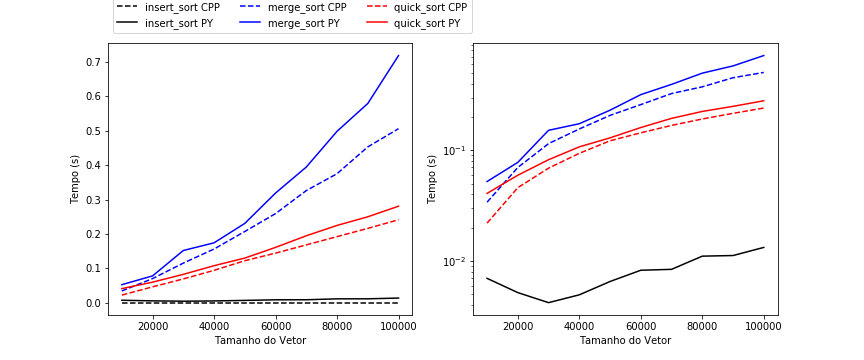
\includegraphics[width=0.8\linewidth,height=5cm]{SortTime_Ascending.png}
    \caption{Comparação de performance dos algoritmos de {\it sorting} para vetores crescentes}
    \vspace{0.5cm}
  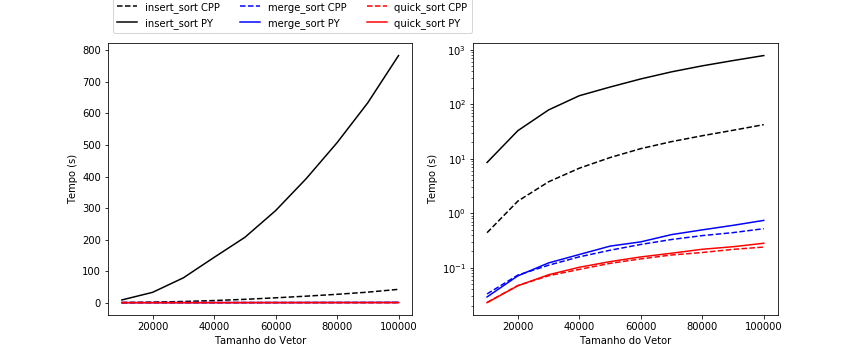
\includegraphics[width=0.8\linewidth,height=5cm]{SortTime_Descending.png}
    \caption{Comparação de performance dos algoritmos de {\it sorting} para vetores decrescentes}
  \end{figure}

  % Figure \ref{fig:boat1} shows a boat.




\end{document}